% -*- coding: utf-8 -*-
% vim: autoindent expandtab tabstop=4 sw=4 sts=4 filetype=tex
% vim: spelllang=de spell
% chktex-file 27 - disable warning about missing include files

\section{Programmablauf}
\label{sec:prototype:sequence}

Nach dem Starten der Applikation erstellt diese die grafische
Benutzeroberfläche und lädt alle externen Shader-Dateien im Unterverzeichnis 
``data''. Die Haupt-Shader-Datei wird als Grundlage für den Ausgabe-Shader
genutzt, die Teil-Shader-Dateien bilden die wählbaren Objekte beziehungsweise
Einträge im Kontextmenü des Graphen.

Nach dem initialen Berechnen und Darstellen der Benutzeroberfläche befindet
sich die Applikation schliesslich in der Hauptschleife. Die Hauptschleife läuft
so lange bis der Benutzer diese mittels Tastendruck auf die Escape-Taste
unterbricht und damit die Applikation beendet.

In der Hauptschleife verarbeitet die Applikation diverse Events wie zum
Beispiel Maus- und Tastatur-Eingaben. Die Verarbeitung findet in der Regel
zuerst in den Kind-Klassen und dann schliesslich in der Hauptklasse statt. Dies
erlaubt es diversen Komponenten, welche eben Kind-Klassen der Applikation sind,
auf Ereignisse, wie zum Beispiel dem Erstellen einer Verbindung zwischen zwei
Knoten, zu reagieren.

Immer wenn ein Knoten dem Haupt-Ausgabeknoten des Graphen direkt oder indirekt
hinzugefügt wird, wird der Graph und somit der Shader neu berechnet
beziehungsweise kompiliert.

Beendet der Benutzer schliesslich die Hauptschleife via Druck auf die
Escape-Taste, so werden alle Ressourcen frei gegeben und die Applikation wird
beendet.

Eine vereinfachte Darstellung des Beschriebenen findet sich in
Abbildung~\ref{fig:prototype:sequence:activity}. Eine detailliertere
Darstellung findet sich in Abbildung~\ref{fig:prototype:sequence:diagram}.

\begin{figure}[H]
    \centering
    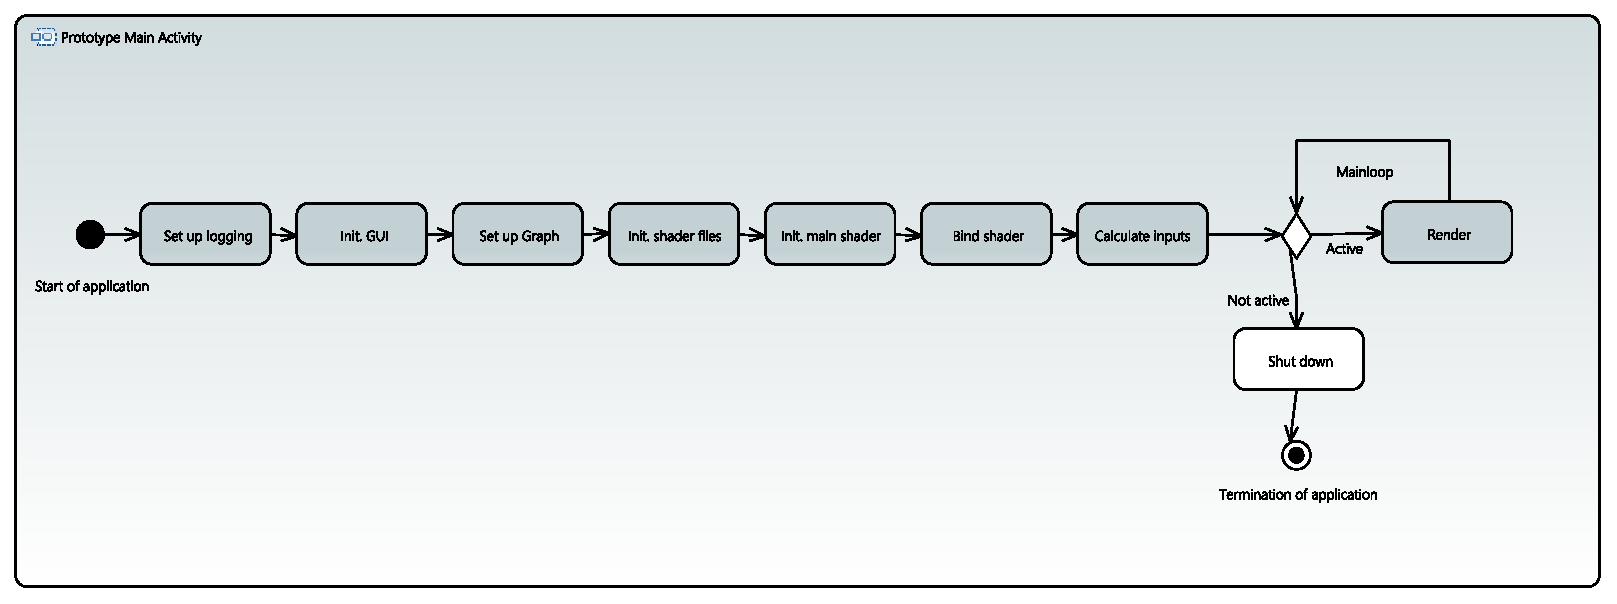
\includegraphics[width=1.0\textwidth]{img/prototype_activity_diagram.PDF}
    \caption{Vereinfachte Darstellung des
        Haupt-Programmablaufes}\label{fig:prototype:sequence:activity}
\end{figure}

\begin{figure}[H]
    \centering
    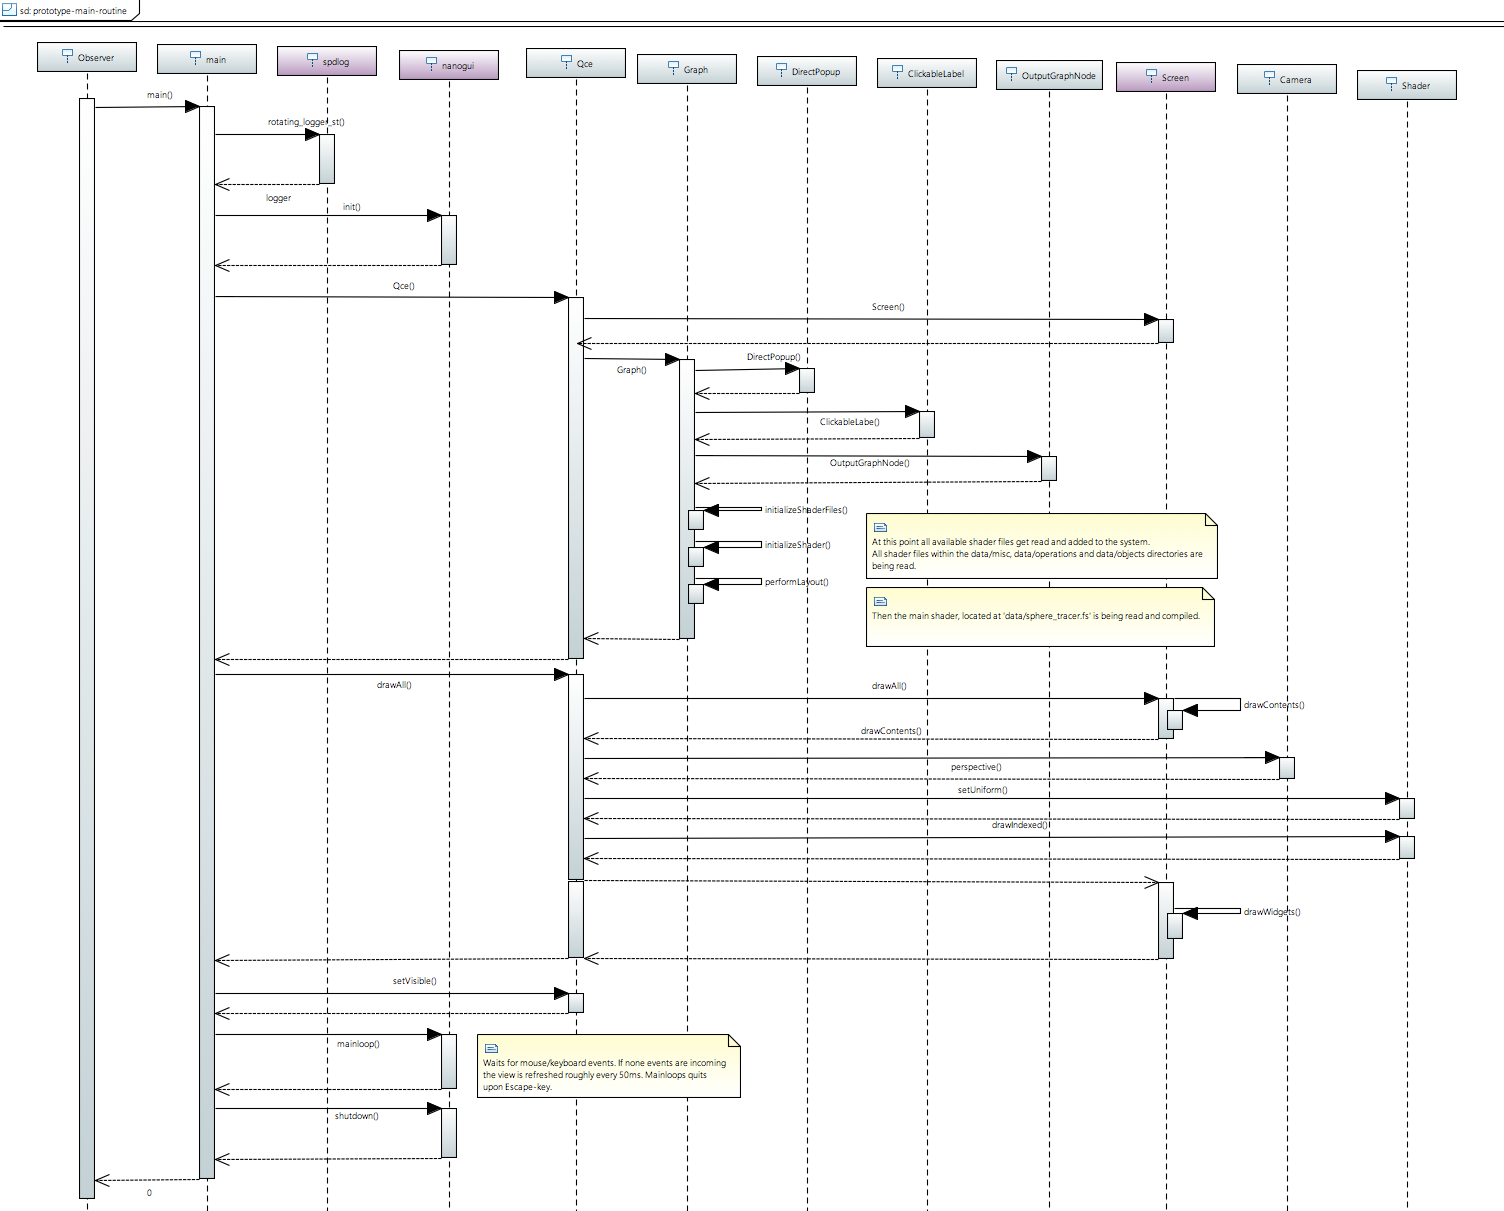
\includegraphics[width=0.9\textwidth]{img/prototype_sequence_diagram.png}
    \caption{Sequenz-Diagramm des Haupt-Ablaufes der
        Prototyp-Applikation}\label{fig:prototype:sequence:diagram}
\end{figure}
